%-------------------------------------------------------------
%---- SOCIAL GOLFERS -----------------------------------------
%-------------------------------------------------------------

\begin{table}[!h]
\centering
\renewcommand{\arraystretch}{1}
\begin{tabular}[t]{|p{3.5cm}|p{10.5cm}|}
	\hline 	
	{\bf Benchmark} & {\sc \sgp}\\
	\hline
	\textbf{Strategy name} & Eager strategy\\
	\hline
	\textbf{Cooperative} & 
	\begin{tabular}[t]{@{}l@{}}
	$\square$ Yes\\
	$\text{\rlap{$\checkmark$}}\square$ No
	\end{tabular}\\
	\hline
	\textbf{Description} & Same solver structure in the \soset{}. Independent multi-walk approach.\\
	\hline
	\textbf{Topology} & 
	\begin{tabular}[t]{@{}l@{}}
	$\vardiamond$ Unconnected (See Figure~\ref{figtop:nc})
	\end{tabular}\\
	\hline
\end{tabular}
%\caption{\sgp}
\label{tab_resume:sgp_eager}
\end{table}

\begin{minipage}{0.5\textwidth}
\centering
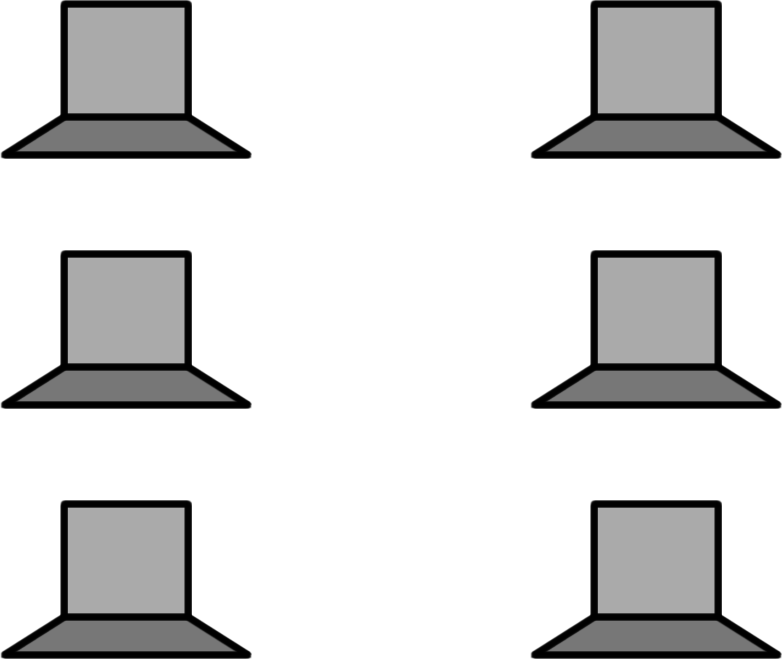
\includegraphics[width=0.5\linewidth]{no_conn.png}
\captionof{figure}{Unconnected}\label{figtop:nc}
\end{minipage}
\begin{minipage}{0.5\textwidth}
\centering
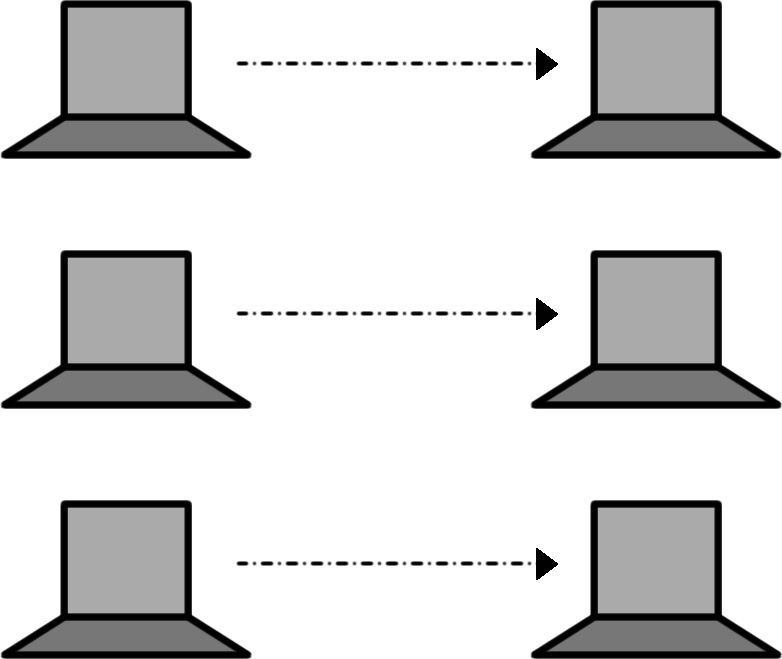
\includegraphics[width=0.5\linewidth]{1-1.png}
\captionof{figure}{Point to point}\label{figtop:1-1}
\end{minipage}

\begin{table}[!h]
\centering
\renewcommand{\arraystretch}{1}
\begin{tabular}[t]{|p{3.5cm}|p{10.5cm}|}
	\hline 	
	{\bf Benchmark} & {\sc \sgp}\\
	\hline
	\textbf{Strategy name} & Simple communication strategy\\
	\hline
	\textbf{Cooperative} & 
	\begin{tabular}[t]{@{}l@{}}
	$\text{\rlap{$\checkmark$}}\square$ Yes\\
	$\square$ No
	\end{tabular}\\
	\hline
	\textbf{Description} & Same solver structure in the \soset{}. Communication in one sense of the current configuration, performed while applying the acceptance criterion of the new configuration for the next iteration.\\
	\hline
	\textbf{Topologies} & 
	\begin{tabular}[t]{@{}l@{}}
	$\vardiamond$ Point to point (See Figure~\ref{figtop:1-1})\\
	$\vardiamond$ Mixed point to point (See Figure~\ref{figtop:mix_1-1})\\
	$\vardiamond$ Bipartition (See Figure~\ref{figtop:1-n})\\
	$\vardiamond$ Mixed bipartition (See Figure~\ref{figtop:mix_1-n})
	\end{tabular}\\
	\hline
\end{tabular}
%\caption{\sgp}
\label{tab_resume:sgp_simple}
\end{table}

\begin{minipage}{0.5\textwidth}
\centering
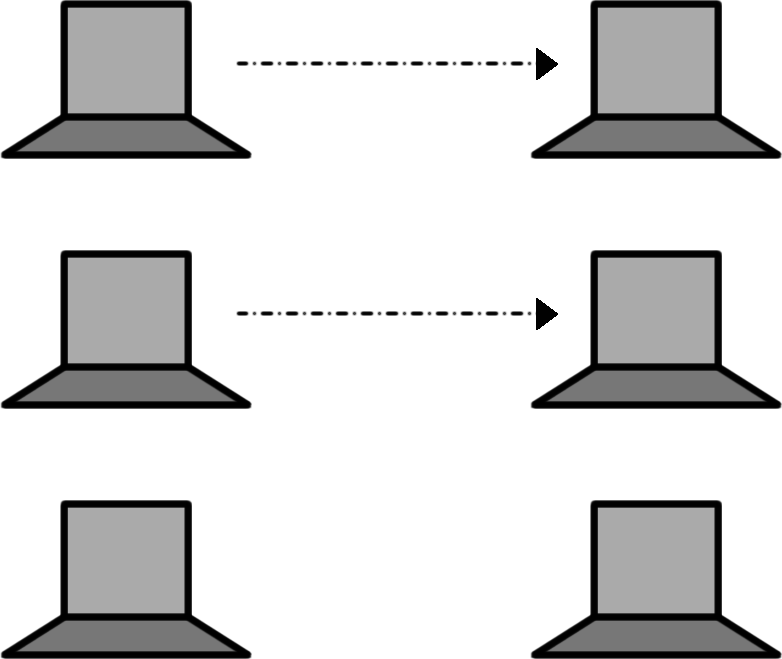
\includegraphics[width=0.5\linewidth]{mix_1-1.png}
\captionof{figure}{Mixed point to point}\label{figtop:mix_1-1}
\end{minipage}
\begin{minipage}{0.5\textwidth}
\centering
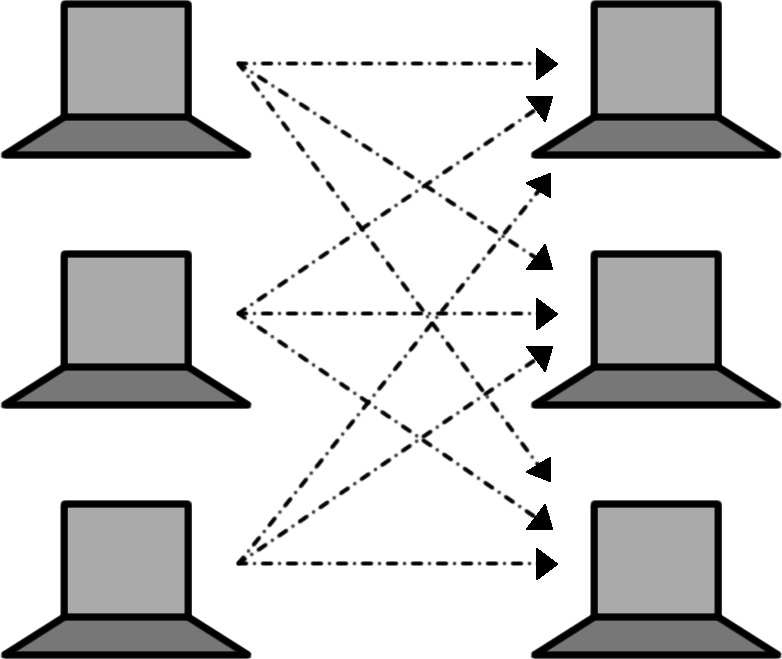
\includegraphics[width=0.5\linewidth]{1-N.png}
\captionof{figure}{Bipartition}\label{figtop:1-n}
\end{minipage}

\begin{minipage}{0.5\textwidth}
\centering
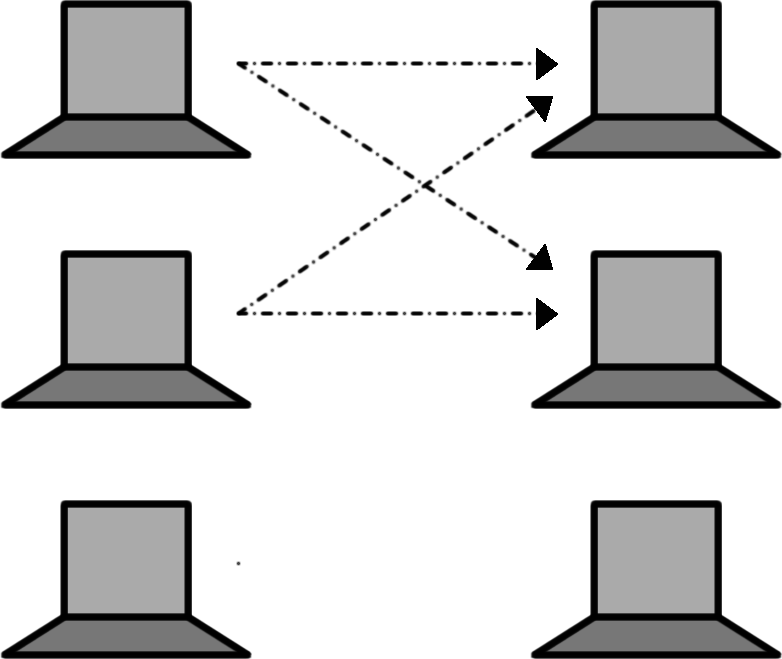
\includegraphics[width=0.5\linewidth]{mix_1-N.png}
\captionof{figure}{Mixed bipartition}\label{figtop:mix_1-n}
\end{minipage}
\begin{minipage}{0.5\textwidth}
\centering
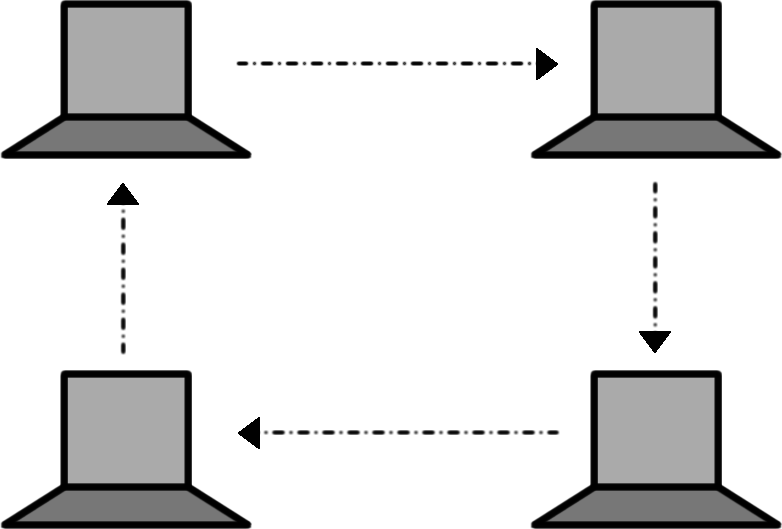
\includegraphics[width=0.5\linewidth]{top_cyc.png}
\captionof{figure}{Ring}\label{figtop:cyc}
\end{minipage}

\begin{table}[!h]
\centering
\renewcommand{\arraystretch}{1}
\begin{tabular}[t]{|p{3.5cm}|p{10.5cm}|}
	\hline 	
	{\bf Benchmark} & {\sc \sgp}\\
	\hline
	\textbf{Strategy name} & Circular exchange strategy\\
	\hline
	\textbf{Cooperative} & 
	\begin{tabular}[t]{@{}l@{}}
	$\text{\rlap{$\checkmark$}}\square$ Yes\\
	$\square$ No
	\end{tabular}\\
	\hline
	\textbf{Description} & Circular communication of the current configuration, performed while applying the acceptance criterion of the new configuration for the next iteration. In each iteration a solver obtains a new derived configurations by modifying a single pre-assigned ``week''. Information exchange takes place after a certain number of iterations. \\
	\hline
	\textbf{Topology} & 
	\begin{tabular}[t]{@{}l@{}}
	$\vardiamond$ Ring (See Figure~\ref{figtop:cyc})
	\end{tabular}\\
	\hline
\end{tabular}
%\caption{\sgp}
\label{tab_resume:sgp_week}
\end{table}

\begin{table}[!h]
\centering
\renewcommand{\arraystretch}{1}
\begin{tabular}[t]{|p{3.5cm}|p{10.5cm}|}
	\hline 	
	{\bf Benchmark} & {\sc \sgp}\\
	\hline
	\textbf{Strategy name} & Dynamic configuration exchange strategy\\
	\hline
	\textbf{Cooperative} & 
	\begin{tabular}[t]{@{}l@{}}
	$\text{\rlap{$\checkmark$}}\square$ Yes\\
	$\square$ No
	\end{tabular}\\
	\hline
	\textbf{Description} & Companion-standard solver communication of the current configuration in one sense, performed while applying the acceptance criterion of the new configuration for the next iteration.\\
	\hline
	\textbf{Topology} & 
	\begin{tabular}[t]{@{}l@{}}
	$\vardiamond$ Cyclic bipartition by groups (See Figure~\ref{figtop:2s_bip})
	\end{tabular}\\
	\hline
\end{tabular}
%\caption{\sgp}
\label{tab_resume:sgp_good}
\end{table}

%\begin{table}[h]
%\centering
%\renewcommand{\arraystretch}{1}
%\begin{tabular}[t]{|p{3.5cm}|p{2.5cm}|p{8cm}|}
%	\hline 	
%	{\bf Benchmark} & \multicolumn{2}{l|}{\sgp}\\
%	\hline
%	\multicolumn{2}{|l|}{\textbf{Communication strategy name}} & Dynamic configuration exchange\\
%	\hline
%	\textbf{Description} & \multicolumn{2}{p{10.5cm}|}{Companion-standard solver communication in one sense of the current configuration, performed while applying the acceptance criterion of the new configuration for the next iteration.}\\
%	\hline
%	\begin{tabular}[t]{@{}l@{}}
%	\textbf{Performance}\\
%	$\text{\rlap{$\checkmark$}}\square$ Success\\
%	$\square$ Moderate success\\
%	$\square$ Not success\\
%	$\square$ Fail
%	\end{tabular}
%	& \multicolumn{2}{p{10.5cm}|}{
%		\begin{tabular}[t]{@{}l@{}}
%			\underline{5--3--7}: 15.63 times faster than sequential approach, \\
%			\hspace{31pt} 2.86 times faster than parallel approach.\\
%			\underline{8--4--7}: 4.29 times faster than sequential approach, \\
%			\hspace{31pt} 2 times faster than parallel approach.\\
%			\underline{9--4--8}: 2.89 times faster than sequential approach, \\
%			\hspace{31pt} 1.67 times faster than parallel approach.\\			
%		\end{tabular}
%		
%	}\\
%	\hline
%\end{tabular}
%%\caption{\sgp}
%\label{tab_resume:sgp_good}
%\end{table}

%\begin{table}[h]
%\centering
%\renewcommand{\arraystretch}{1}
%\begin{tabular}[t]{|p{3.5cm}|p{2.5cm}|p{8cm}|}
%	\hline 	
%	{\bf Benchmark} & \multicolumn{2}{l|}{\sgp}\\
%	\hline
%	\multicolumn{2}{|l|}{\textbf{Communication strategy name}} & Dynamic configuration exchange\\
%	\hline
%	\textbf{Description} & \multicolumn{2}{p{10.5cm}|}{Companion-standard solver communication in one sense of the current configuration, performed while applying the acceptance criterion of the new configuration for the next iteration.}\\
%	\hline
%	\begin{tabular}[t]{@{}l@{}}
%	\textbf{Performance}\\
%	$\text{\rlap{$\checkmark$}}\square$ Success\\
%	$\square$ Moderate success\\
%	$\square$ Not success\\
%	$\square$ Fail
%	\end{tabular}
%	& \multicolumn{2}{p{10.5cm}|}{
%		\begin{tabular}[t]{@{}l@{}}
%			\underline{5--3--7}: 15.63 times faster than sequential approach, \\
%			\hspace{31pt} 2.86 times faster than parallel approach.\\
%			\underline{8--4--7}: 4.29 times faster than sequential approach, \\
%			\hspace{31pt} 2 times faster than parallel approach.\\
%			\underline{9--4--8}: 2.89 times faster than sequential approach, \\
%			\hspace{31pt} 1.67 times faster than parallel approach.\\			
%		\end{tabular}
%		
%	}\\
%	\hline
%\end{tabular}
%%\caption{\sgp}
%\label{tab_resume:sgp_good}
%\end{table}

\begin{minipage}{0.5\textwidth}
\centering
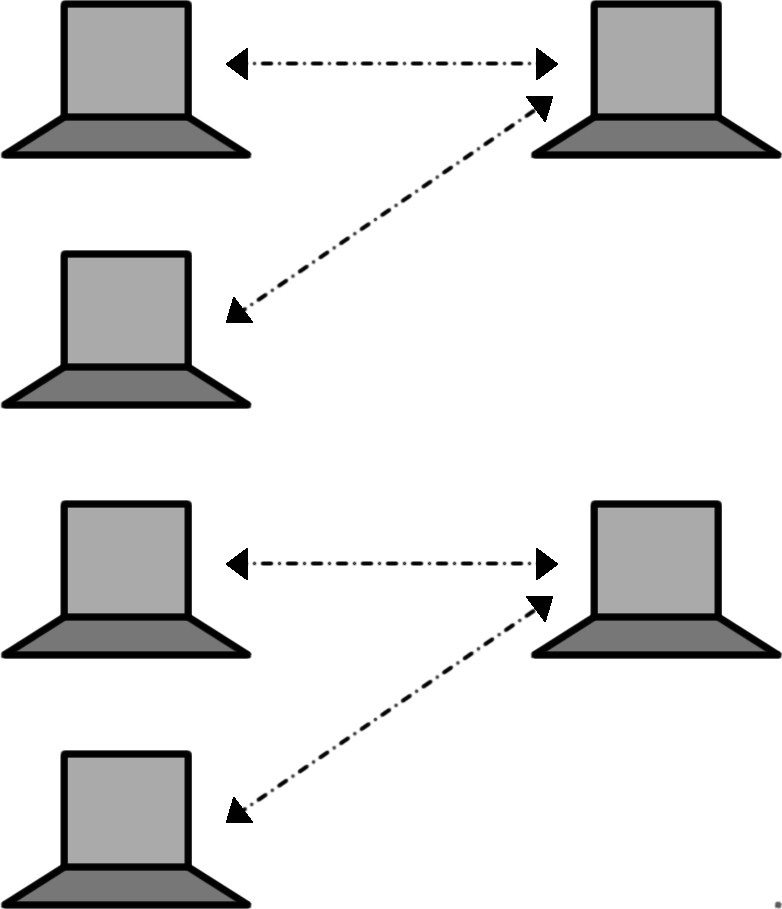
\includegraphics[width=0.5\linewidth]{2S_N-1.png}
\captionof{figure}{Cyclic bipartition by groups}\label{figtop:2s_bip}
\end{minipage}
\begin{minipage}{0.5\textwidth}
\centering
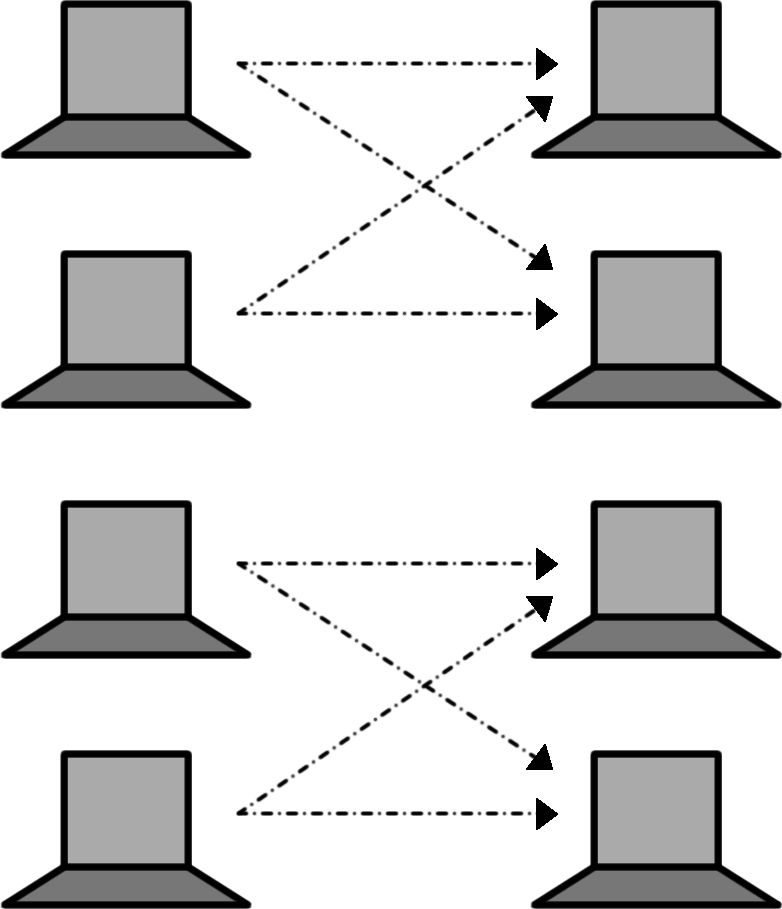
\includegraphics[width=0.5\linewidth]{group_1-N.png}
\captionof{figure}{Bipartition by groups}\label{figtop:gr_bip}
\end{minipage}

%-------------------------------------------------------------
%---- N_QUEENS -----------------------------------------------
%-------------------------------------------------------------

\begin{table}[!h]
\centering
\renewcommand{\arraystretch}{1}
\begin{tabular}[t]{|p{3.5cm}|p{10.5cm}|}
	\hline 	
	{\bf Benchmark} & {\sc \nqp}\\
	\hline
	\textbf{Strategy name} & Simple parallel strategy\\
	\hline
	\textbf{Cooperative} & 
	\begin{tabular}[t]{@{}l@{}}
	$\square$ Yes\\
	$\text{\rlap{$\checkmark$}}\square$ No
	\end{tabular}\\
	\hline
	\textbf{Description} & Same solver structure in the \soset{}. Independent multi-walk approach.\\
	\hline
	\textbf{Topology} &
	\begin{tabular}[t]{@{}l@{}}
	$\vardiamond$ Unconnected %(See Figure~\ref{figtop:nc})
	\end{tabular}\\
	\hline
\end{tabular}
%\caption{\sgp}
\label{tab_resume:nqp_simple}
\end{table}

\begin{table}[!h]
\centering
\renewcommand{\arraystretch}{1}
\begin{tabular}[t]{|p{3.5cm}|p{10.5cm}|}
	\hline 	
	{\bf Benchmark} & {\sc \nqp}\\
	\hline
	\textbf{Strategy name} & Simple communication strategy\\
	\hline
	\textbf{Cooperative} & 
	\begin{tabular}[t]{@{}l@{}}
	$\text{\rlap{$\checkmark$}}\square$ Yes\\
	$\square$ No
	\end{tabular}\\
	\hline
	\textbf{Description} & Same solver structure in the \soset{}. Communication in one sense of the current configuration, performed while applying the acceptance criterion of the new configuration for the next iteration.\\
	\hline
	\textbf{Topologies} & 
	\begin{tabular}[t]{@{}l@{}}
	$\vardiamond$ Point to point \\% (See Figure~\ref{figtop:1-1})\\
	$\vardiamond$ Bipartition \\%(See Figure~\ref{figtop:1-n})\\
	$\vardiamond$ Bipartition by groups 
	\end{tabular}\\
	\hline
\end{tabular}
%\caption{\sgp}
\label{tab_resume:nqp_simple_com}
\end{table}

\begin{table}[!h]
\centering
\renewcommand{\arraystretch}{1}
\begin{tabular}[t]{|p{3.5cm}|p{10.5cm}|}
	\hline 	
	{\bf Benchmark} & {\sc \nqp}\\
	\hline
	\textbf{Strategy name} & Cyclic configuration exchange strategy\\
	\hline
	\textbf{Cooperative} & 
	\begin{tabular}[t]{@{}l@{}}
	$\text{\rlap{$\checkmark$}}\square$ Yes\\
	$\square$ No
	\end{tabular}\\
	\hline
	\textbf{Description} & Companion-standard solver communication of the current configuration in both senses, performed while applying the acceptance criterion of the new configuration for the next iteration.\\
	\hline
	\textbf{Topologies} & 
	\begin{tabular}[t]{@{}l@{}}
	$\vardiamond$ Cyclic point to point (See Figure~\ref{figtop:cyc_1-1})\\
	$\vardiamond$ Cyclic bipartition by groups \\
	\end{tabular}\\
	\hline
\end{tabular}
%\caption{\sgp}
\label{tab_resume:nqp_good}
\end{table}

\begin{figure}[!h]
\centering
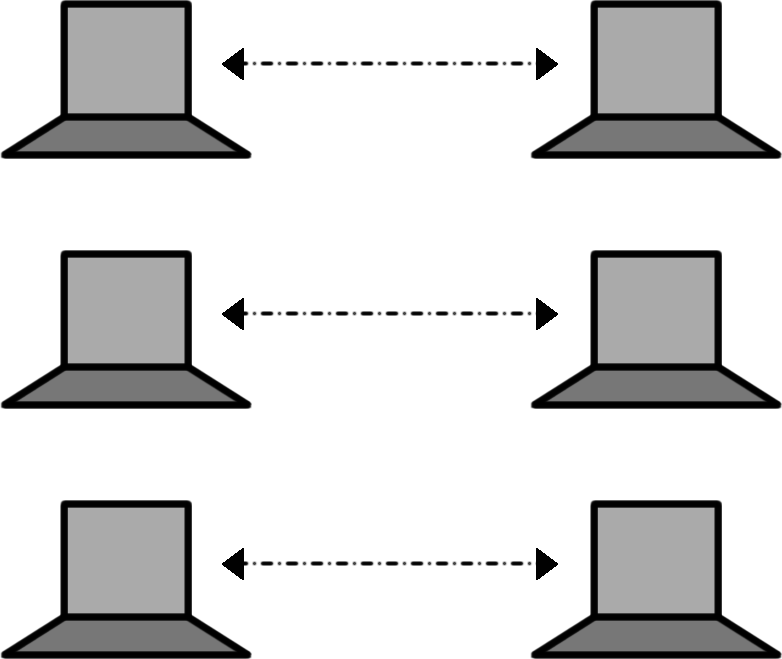
\includegraphics[width=0.25\linewidth]{2S_1-1.png}
\caption{Cyclic point to point}\label{figtop:cyc_1-1}
\end{figure}

%\begin{table}[h]
%\centering
%\renewcommand{\arraystretch}{1}
%\begin{tabular}[t]{|p{3.5cm}|p{2.5cm}|p{8cm}|}
%	\hline 	
%	{\bf Benchmark} & \multicolumn{2}{l|}{\nqp}\\
%	\hline
%	\multicolumn{2}{|l|}{\textbf{Communication strategy name}} & Simple \commstr\\
%	\hline
%	\textbf{Description} & \multicolumn{2}{p{10.5cm}|}{Same solver structure in the \soset{}. Communication in one sense of the current configuration, performed while applying the acceptance criterion of the new configuration for the next iteration.}\\
%	\hline
%	\begin{tabular}[t]{@{}l@{}}
%	\textbf{Performance}\\
%	$\square$ Success\\
%	$\text{\rlap{$\checkmark$}}\square$ Moderate success\\
%	$\square$ Not success\\
%	$\square$ Fail
%	\end{tabular}
%	& \multicolumn{2}{p{10.5cm}|}{
%		\begin{tabular}[t]{@{}l@{}}
%			\underline{250}: 1.60 times faster than sequential approach, \\
%			\hspace{21pt} 1.26 times faster than parallel approach.\\
%			\underline{500}: 1.94 times faster than sequential approach, \\
%			\hspace{21pt} 1.33 times faster than parallel approach.\\
%			\underline{1000}: 1.52 times faster than sequential approach, \\
%			\hspace{26pt} 1.30 times faster than parallel approach.\\
%			\underline{3000}: 1.25 times faster than sequential approach, \\
%			\hspace{26pt} 1.10 times faster than parallel approach.\\
%			\underline{6000}: 1.09 times faster than sequential approach, \\
%			\hspace{26pt} 1.06 times faster than parallel approach.\\
%		\end{tabular}		
%	}\\
%	\hline
%\end{tabular}
%%\caption{\sgp}
%\label{tab_resume:nqp_simple}
%\end{table}

%\begin{table}[h]
%\centering
%\renewcommand{\arraystretch}{1}
%\begin{tabular}[t]{|p{3.5cm}|p{2.5cm}|p{8cm}|}
%	\hline 	
%	{\bf Benchmark} & \multicolumn{2}{l|}{\nqp}\\
%	\hline
%	\multicolumn{2}{|l|}{\textbf{Communication strategy name}} & Cyclic \commstr\\
%	\hline
%	\textbf{Description} & \multicolumn{2}{p{10.5cm}|}{Cyclic companion-standard solver communication of the current configuration, performed while applying the acceptance criterion of the new configuration for the next iteration.}\\
%	\hline
%	\begin{tabular}[t]{@{}l@{}}
%	\textbf{Performance}\\
%	$\text{\rlap{$\checkmark$}}\square$ Success\\
%	$\square$ Moderate success\\
%	$\square$ Not success\\
%	$\square$ Fail
%	\end{tabular}
%	& \multicolumn{2}{p{10.5cm}|}{
%		\begin{tabular}[t]{@{}l@{}}
%			\underline{250}: 3.22 times faster than sequential approach, \\
%			\hspace{21pt} 2.11 times faster than parallel approach.\\
%			\underline{500}: 2.50 times faster than sequential approach, \\
%			\hspace{21pt} 1.71 times faster than parallel approach.\\
%			\underline{1000}: 1.67 times faster than sequential approach, \\
%			\hspace{26pt} 1.43 times faster than parallel approach.\\
%			\underline{3000}: 1.47 times faster than sequential approach, \\
%			\hspace{26pt} 1.30 times faster than parallel approach.\\
%			\underline{6000}: 1.12 times faster than sequential approach, \\
%			\hspace{26pt} 1.08 times faster than parallel approach.\\
%		\end{tabular}		
%	}\\
%	\hline
%\end{tabular}
%%\caption{\sgp}
%\label{tab_resume:nqp_good}
%\end{table}

%-------------------------------------------------------------
%---- COSTAS ARRAY -------------------------------------------
%-------------------------------------------------------------

\begin{table}[!h]
\centering
\renewcommand{\arraystretch}{1}
\begin{tabular}[t]{|p{3.5cm}|p{10.5cm}|}
	\hline 	
	{\bf Benchmark} & {\sc \carrp}\\
	\hline
	\textbf{Strategy name} & Simple parallel strategy\\
	\hline
	\textbf{Cooperative} & 
	\begin{tabular}[t]{@{}l@{}}
	$\square$ Yes\\
	$\text{\rlap{$\checkmark$}}\square$ No
	\end{tabular}\\
	\hline
	\textbf{Description} & Same solver structure in the \soset{}. Independent multi-walk approach.\\
	\hline
	\textbf{Topology} &
	\begin{tabular}[t]{@{}l@{}}
	$\vardiamond$ Unconnected %(See Figure~\ref{figtop:nc})
	\end{tabular}\\
	\hline	
\end{tabular}
%\caption{\sgp}
\label{tab_resume:cap_simple}
\end{table}

\begin{table}[!h]
\centering
\renewcommand{\arraystretch}{1}
\begin{tabular}[t]{|p{3.5cm}|p{10.5cm}|}
	\hline 	
	{\bf Benchmark} & {\sc \carrp}\\
	\hline
	\textbf{Strategy name} & Simple communication strategy (variant A)\\
	\hline
	\textbf{Cooperative} & 
	\begin{tabular}[t]{@{}l@{}}
	$\text{\rlap{$\checkmark$}}\square$ Yes\\
	$\square$ No
	\end{tabular}\\
	\hline
	\textbf{Description} & Same solver structure in the \soset{}. Communication in one sense of the current configuration, performed while applying the acceptance criterion of the new configuration for the next iteration.\\
	\hline
	\textbf{Topologies} &
	\begin{tabular}[t]{@{}l@{}}
	$\vardiamond$ Point to point \\
	$\vardiamond$ Bipartition \\
	\end{tabular}\\
	\hline
\end{tabular}
%\caption{\sgp}
\label{tab_resume:cap_A}
\end{table}

\begin{table}[!h]
\centering
\renewcommand{\arraystretch}{1}
\begin{tabular}[t]{|p{3.5cm}|p{10.5cm}|}
	\hline 	
	{\bf Benchmark} & {\sc \carrp}\\
	\hline
	\textbf{Strategy name} & Simple communication strategy (variant B)\\
	\hline
	\textbf{Cooperative} & 
	\begin{tabular}[t]{@{}l@{}}
	$\text{\rlap{$\checkmark$}}\square$ Yes\\
	$\square$ No
	\end{tabular}\\
	\hline
	\textbf{Description} & Same solver structure in the \soset{}. Communication in one sense of the current configuration, performed while applying the \textit{reset}.\\
	\hline
	\textbf{Topologies} &
	\begin{tabular}[t]{@{}l@{}}
	$\vardiamond$ Point to point \\
	$\vardiamond$ Bipartition \\
	\end{tabular}\\
	\hline	
\end{tabular}
%\caption{\sgp}
\label{tab_resume:cap_B}
\end{table}

%-------------------------------------------------------------
%---- GOLOMB RULER -------------------------------------------
%-------------------------------------------------------------

\begin{table}[!h]
\centering
\renewcommand{\arraystretch}{1}
\begin{tabular}[t]{|p{3.5cm}|p{10.5cm}|}
	\hline 	
	{\bf Benchmark} & {\sc \grp}\\
	\hline
	\textbf{Strategy name} & Simple parallel strategy\\
	\hline
	\textbf{Cooperative} & 
	\begin{tabular}[t]{@{}l@{}}
	$\square$ Yes\\
	$\text{\rlap{$\checkmark$}}\square$ No
	\end{tabular}\\
	\hline
	\textbf{Description} & Same solver structure in the \soset{}. Independent multi-walk approach.\\
	\hline
	\textbf{Topology} &
	\begin{tabular}[t]{@{}l@{}}
	$\vardiamond$ Unconnected %(See Figure~\ref{figtop:nc})
	\end{tabular}\\	
	\hline
\end{tabular}
%\caption{\sgp}
\label{tab_resume:grp_simple_nota}
\end{table}

\begin{table}[!h]
\centering
\renewcommand{\arraystretch}{1}
\begin{tabular}[t]{|p{3.5cm}|p{10.5cm}|}
	\hline 	
	{\bf Benchmark} & {\sc \grp}\\
	\hline
	\textbf{Strategy name} & Tabu-list parallel strategy\\
	\hline
	\textbf{Cooperative} & 
	\begin{tabular}[t]{@{}l@{}}
	$\square$ Yes\\
	$\text{\rlap{$\checkmark$}}\square$ No
	\end{tabular}\\
	\hline
	\textbf{Description} & Same solver structure in the \soset{}, using a tabo list. Independent multi-walk approach.\\
	\hline
	\textbf{Topology} &
	\begin{tabular}[t]{@{}l@{}}
	$\vardiamond$ Unconnected %(See Figure~\ref{figtop:nc})
	\end{tabular}\\
	\hline
\end{tabular}
%\caption{\sgp}
\label{tab_resume:grp_simple_ta}
\end{table}

\begin{table}[!h]
\centering
\renewcommand{\arraystretch}{1}
\begin{tabular}[t]{|p{3.5cm}|p{10.5cm}|}
	\hline 	
	{\bf Benchmark} & {\sc \grp}\\
	\hline
	\textbf{Strategy name} & Local minima evasion strategy\\
	\hline
	\textbf{Cooperative} & 
	\begin{tabular}[t]{@{}l@{}}
	$\text{\rlap{$\checkmark$}}\square$ Yes\\
	$\square$ No
	\end{tabular}\\
	\hline
	\textbf{Description} & Same solver structure in the \soset{}. Communication in one sense of the current configuration, performed by the sender when this current configuration is classified as a local minima (after a number of iterations without improving the current cost), and by the receiver while performing the restart.\\
	\hline
	\textbf{Topologies} &
	\begin{tabular}[t]{@{}l@{}}
	$\vardiamond$ Point to point \\
	$\vardiamond$ Bipartition \\
	\end{tabular}\\
	\hline	
\end{tabular}
%\caption{\sgp}
\label{tab_resume:grp_comm}
\end{table}